\documentclass{article}
\usepackage[utf8]{inputenc}

\title{EE2703 Applied Programming Lab \\ Assignment 8}
\author{
  \textbf{Name}: Neham Hitesh Jain\\
  \textbf{Roll Number}: EE19B084
}\date{April 23, 2021}

\usepackage{listings}
\usepackage{natbib}
\usepackage{geometry} % Used to adjust the document margins
\usepackage{amsmath}
\usepackage{subfig}
\usepackage{verbatim}
\usepackage{color}
\usepackage{graphicx}
\definecolor{dkgreen}{rgb}{0,0.6,0}
\definecolor{gray}{rgb}{0.5,0.5,0.5}
\definecolor{mauve}{rgb}{0.58,0,0.82}

\lstset{frame=tb,
  language=Python,
  aboveskip=3mm,
  belowskip=3mm,
  showstringspaces=false,
  columns=flexible,
  basicstyle={\small\ttfamily},
  numbers=none,
  numberstyle=\tiny\color{gray},
  keywordstyle=\color{blue},
  commentstyle=\color{dkgreen},
  stringstyle=\color{mauve},
  breaklines=true,
  breakatwhitespace=true,
  tabsize=3
}

\geometry{verbose,tmargin=1in,bmargin=1in,lmargin=1.5in,rmargin=1.5in}

\begin{document}

\maketitle
\newpage

\begin{abstract}
    In this assignment, we use Sympy to analytically solve a matrix equation
    governing an analog circuit. We look at two circuits, an active low pass
    filter and an active high pass filter. We create matrices using node
    equations for the circuits in sympy, and then solve the equations
    analytically. We then convert the resulting sympy solution into a numpy
    function which can be called. We then use the signals toolbox we studied
    in the last assignment to understand the responses of the two circuits
    to various inputs.
\end{abstract}


\section*{Low Pass Filter}
Consider the circuit given below,


\begin{figure}[!tbh]
   	\centering
   	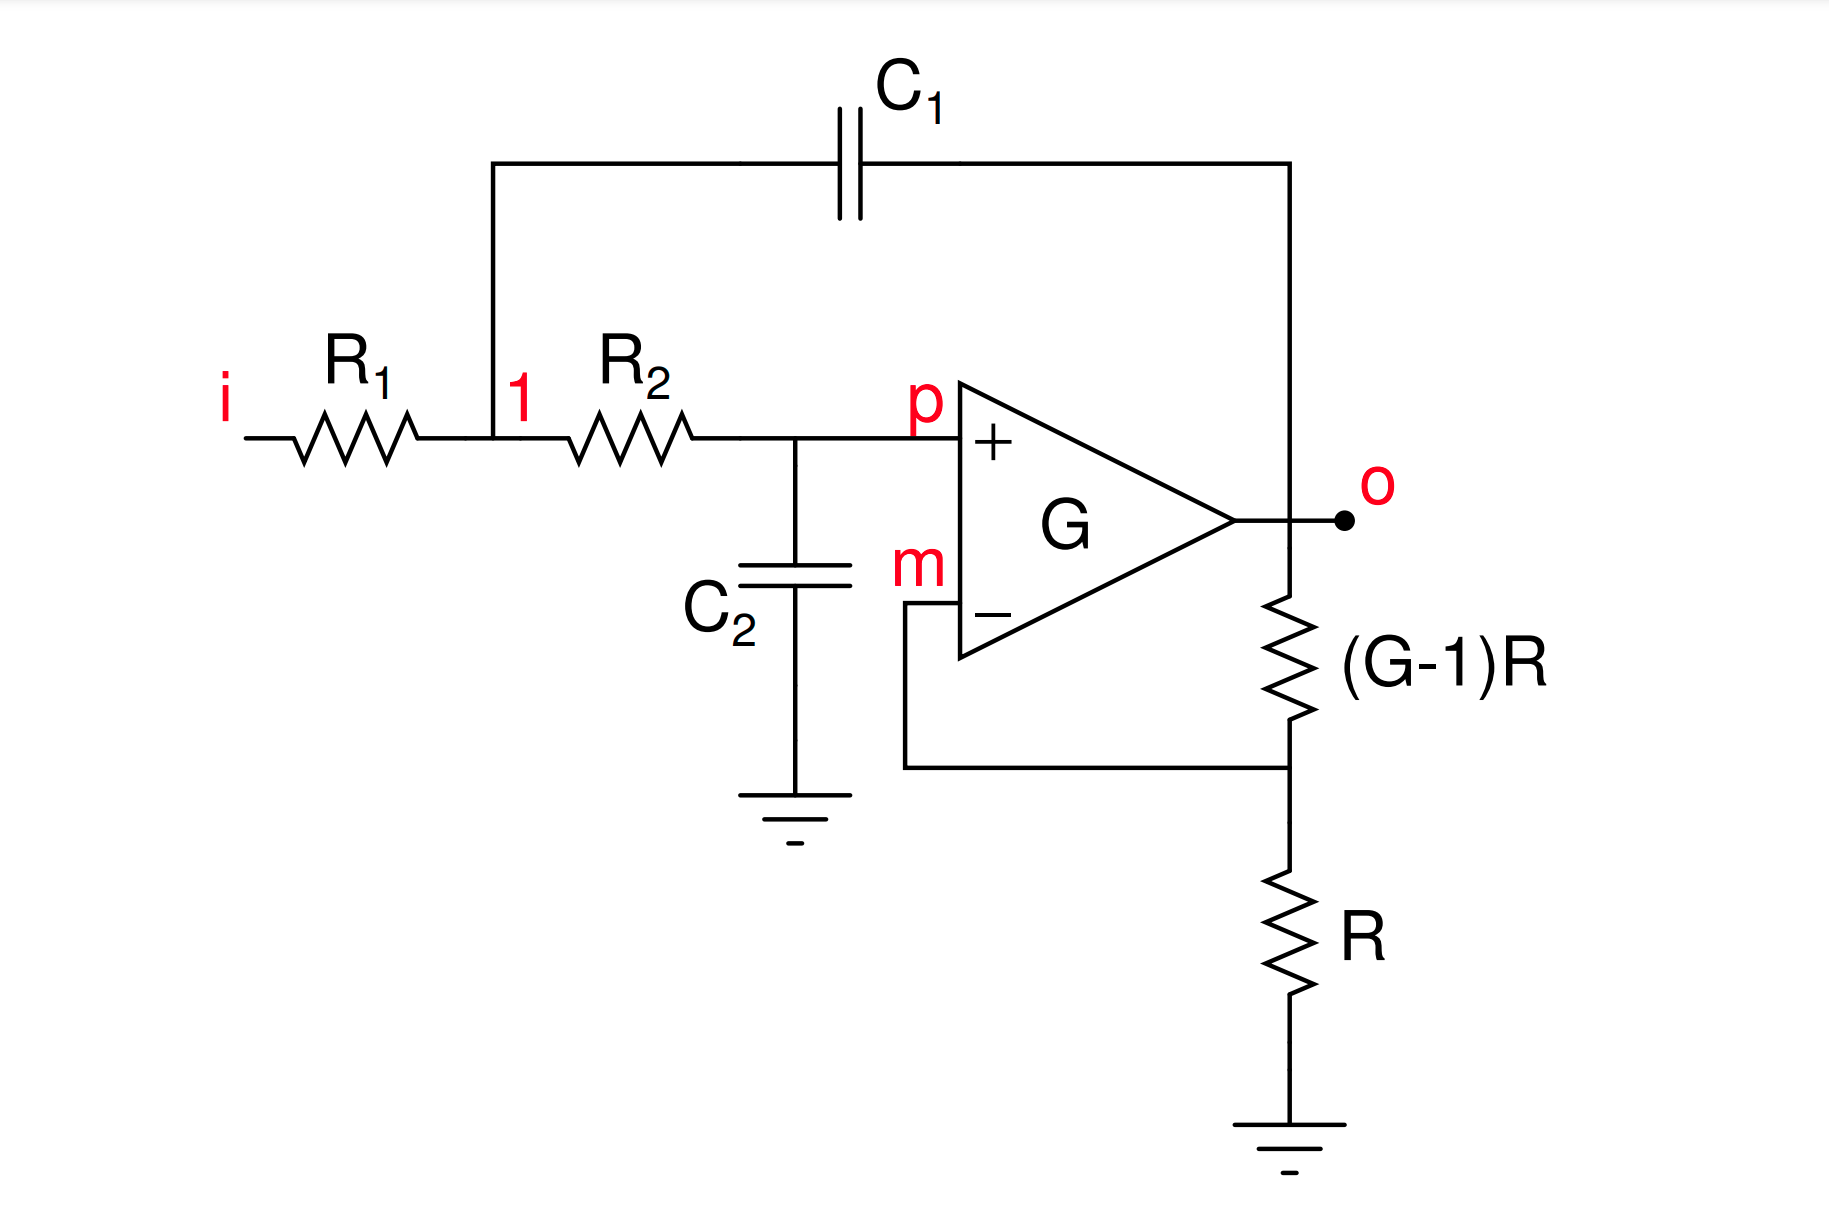
\includegraphics[scale=0.1]{plots/low_pass.png}   
   	\caption{Low Pass Filter Circuit}
   	\label{fig:Figure_1}
   \end{figure}

\noindent
The above circuit gives the following matrix after simplification of Modified Nodal Equations.
\\
\begin{equation*}
    \begin{bmatrix}
    0   & 0 & 1  & -1/G \\
    \frac{-1}{sR_2C_2}  & 1 & 0 & 0\\
    0  & -G & G & 1 \\
    \frac{-1}{R_1} - \frac{1}{R_2} - s*C_1 & \frac{1}{R_2} & 0 & sC_1
\end{bmatrix}
\begin{bmatrix}
    V_1\\
    V_p\\
    V_m \\
    V_o
\end{bmatrix}
=
\begin{bmatrix}
    0 \\
    0 \\
    0 \\
    \frac{-V_i(s)}{R_1} \\
\end{bmatrix}
\end{equation*}

\begin{lstlisting}
def lowpass(R1=10e3,R2=10e3,C1=1e-9,C2=1e-9,G=1.586,Vi=1,s=symbols('s')):
    """Solve the given lowpass filter circuit for a given input Vi."""

    A=Matrix([[0,0,1,-1/G],
                [-1/(1+s*R2*C2),1,0,0],
                [0,-G,G,1],
                [-1/R1-1/R2-s*C1,1/R2,0,s*C1]])

    b=Matrix([0,0,0,-Vi/R1])    
    V=A.inv()*b

    return V
\end{lstlisting}

\subsection*{Magnitude response}
The magnitude response of the circuit is,
\newpage
\begin{lstlisting}
def get_bode_plot(H,title):
    ''' Plots the magnitude and phase response of a given transfer function '''

    w, mag, phase = H.bode()
    #Plotting Magnitude Response of Transfer Function 
    p = General_Plotter("Frequency in rad/s (log)","Magnitude in dB","Magnitude plot"+title)
    p.semilogx(w,mag)
    
    #Phase Response of Transfer Function
    p = General_Plotter("Frequency in rad/s (log)","Phase in degrees","Phase plot"+title)
    p.semilogx(w,phase)
\end{lstlisting}


\begin{figure}%
    \centering
    \subfloat[\centering Magnitude Plot]{{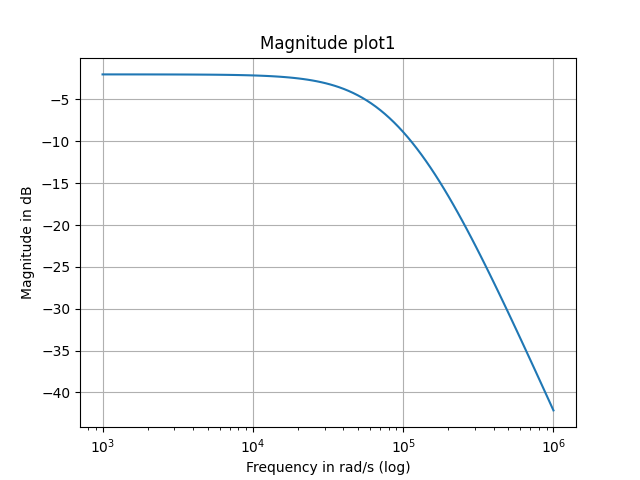
\includegraphics[width=6cm]{plots/Magnitude plot1.png} }}%
    \qquad
    \subfloat[\centering Phase Plot]{{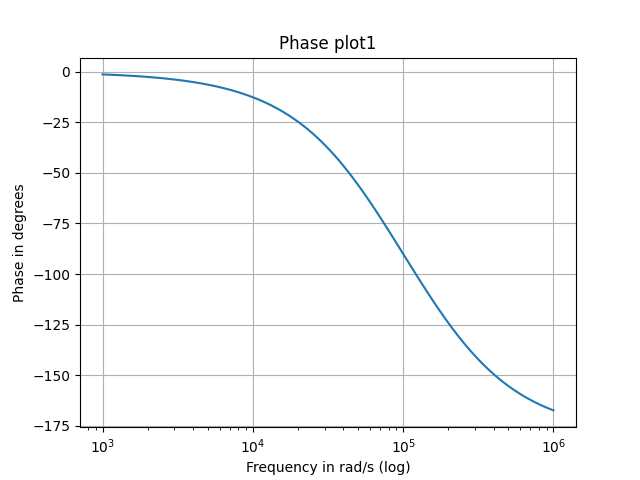
\includegraphics[width=6cm]{plots/Phase plot1.png} }}%
    \caption{Bode Plot of Low Pass Circuit}%
    \label{fig:example}%
\end{figure}

Clearly, the circuit acts as a low pass filter as the magnitude response drops rapidly after a certain frequency.


\section*{High Pass Filter}
Consider the circuit below,
\begin{figure}[!tbh]
   	\centering
   	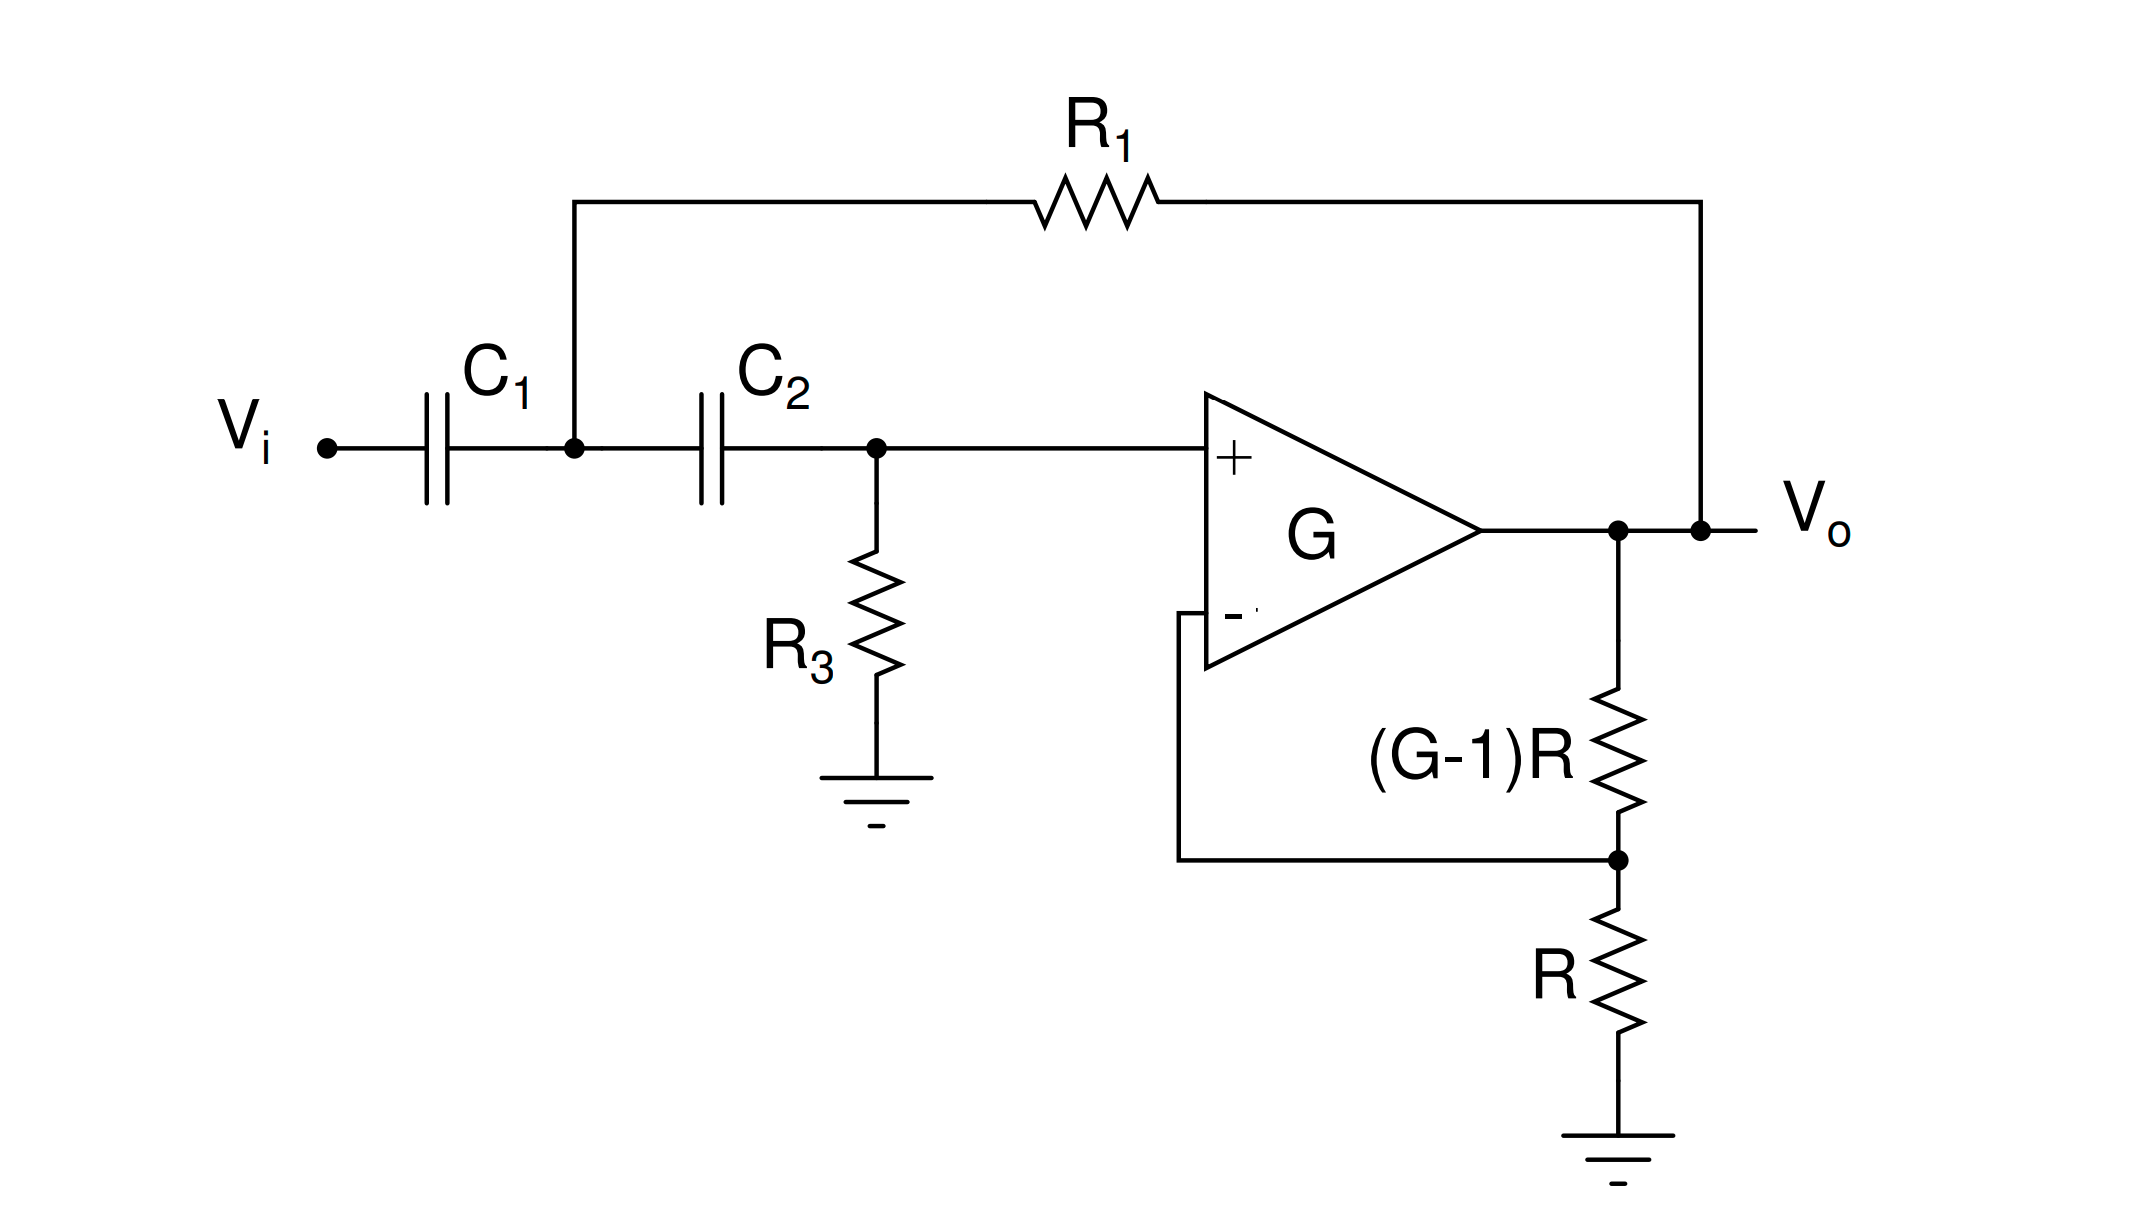
\includegraphics[scale=0.1]{plots/high_pass.png}   
   	\caption{High Pass Filter Circuit}
   	\label{fig:Figure_3}
   \end{figure}
The above circuit gives the following matrix after simplification of Modified Nodal Equations.
\begin{equation*}
    \begin{bmatrix}
    0   & -1 & 0  & 1/G \\
    \frac{s*C_2*R_3}{1+s*C_2*R_3}  & 0 & -1 & 0\\
    0  & G & -G & 1 \\
    -s*C_2 - \frac{1}{R_1} - s*C_1 & 0 & s*C_2 & \frac{1}{R_1}
\end{bmatrix}
\begin{bmatrix}
    V_1\\
    V_p\\
    V_m \\
    V_o
\end{bmatrix}
=
\begin{bmatrix}
    0 \\
    0 \\
    0 \\
    -V_i(s)*s*C_1 \\
    
\end{bmatrix}
\end{equation*}

\subsection*{Magnitude response}
The magnitude response of the circuit is:
\\
\begin{lstlisting}
#Step Response of the Highpass Circuit
V_h = highpass()[3]
H2 = sympy_to_lti(V_h)
get_bode_plot(H2,title="2")
\end{lstlisting}

\begin{figure}[!tbh]
    \centering
    \subfloat[\centering Magnitude Plot]{{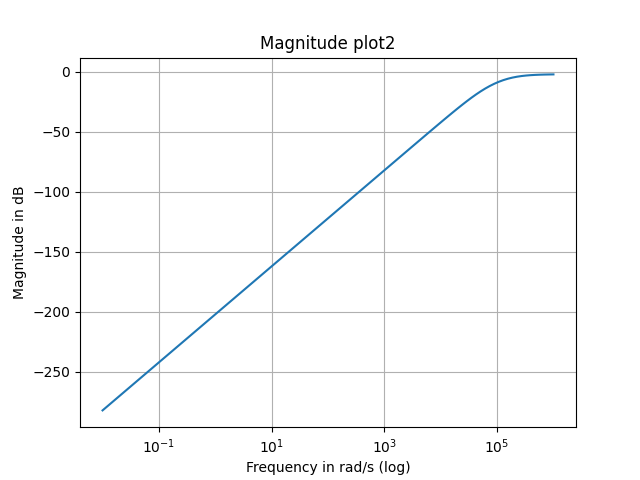
\includegraphics[width=6cm]{plots/Magnitude plot2.png} }}%
    \qquad
    \subfloat[\centering Phase Plot]{{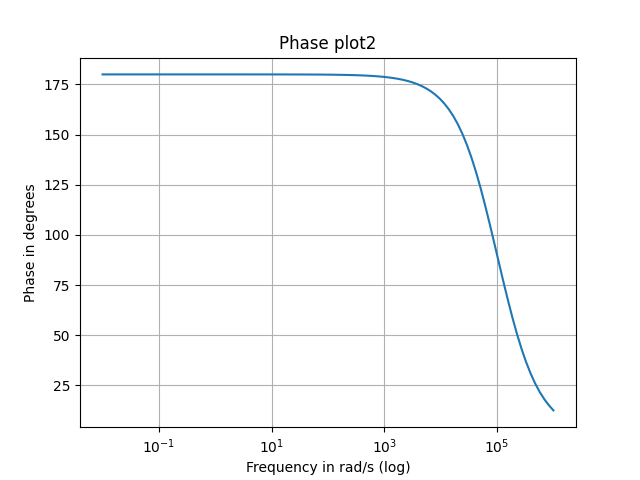
\includegraphics[width=6cm]{plots/Phase plot2.png} }}%
    \caption{Bode Plot of High Pass Circuit}%
    \label{fig:example2}%
\end{figure}
\noindent
Clearly, the circuit acts as a high pass filter as the magnitude response starts with low values and then increases and remains constant with frequency after a certain cut-off frequency.

\section{Converting Sympy to Scipy}
On obtaining the transfer function in it's symbolic representation, we now convert it to a form that can be used by Scipy's Signals package.

\begin{lstlisting}
def sympy_to_lti(xpr, s=symbols('s')):
    """ Convert Sympy transfer function polynomial to Scipy LTI """

    num, den = simplify(xpr).as_numer_denom()  # returns the expressions
    p_num_den = poly(num, s), poly(den, s)
    num,den = p_num_den[0].all_coeffs(), p_num_den[1].all_coeffs()

    num=list(map(float, num))
    den=list(map(float, den))

    return sp.lti(num, den)

\end{lstlisting}

\section*{Step Response}
We plot the outputs of the two systems to a unit step below:

\begin{verbatim}
Steady state value of low pass filter step response: 0.7930
Steady state value of high pass filter step response: 0.0000
Initial value of low pass filter step response: 0.0000
Initial value of high pass filter step response: 0.7930
\end{verbatim}

\begin{figure}%
    \centering
    \subfloat[\centering Low Pass Filter Circuit]{{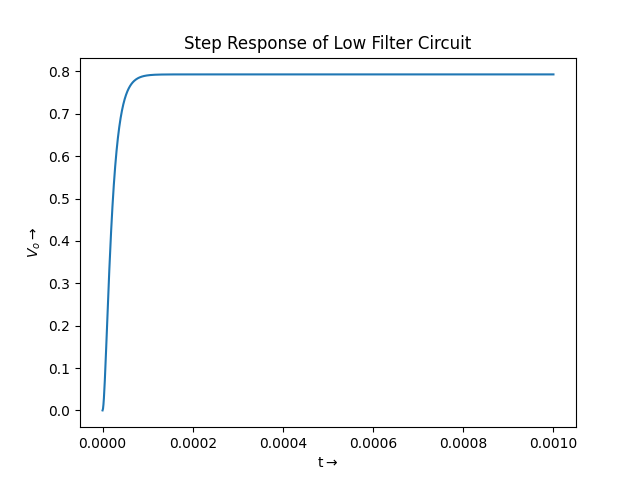
\includegraphics[width=6cm]{plots/Step Response of Low Filter Circuit.png} }}%
    \qquad
    \subfloat[\centering High Pass Filter Circuit]{{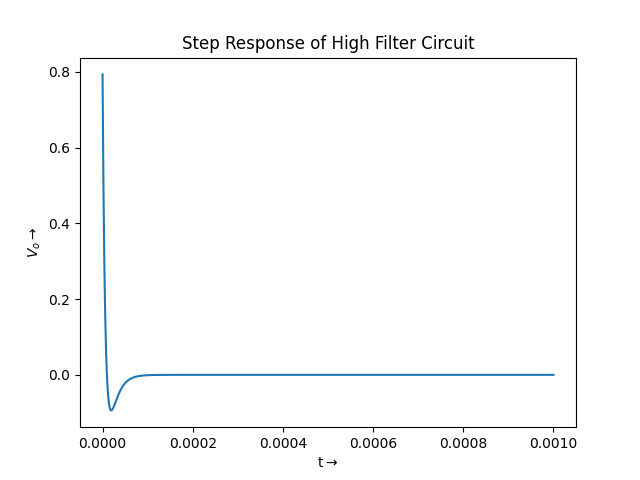
\includegraphics[width=6cm]{plots/Step Response of High Filter Circuit.png} }}%
    \caption{Step Response}%
    \label{Figure 4}
\end{figure}
		
\begin{itemize}
    \item
      We observe that the low pass filter inverts the step and attenuates it
      by a factor of \(0.793\). We
      observe a transient which decays quite fast, again as we expected as
      the system is almost critically damped.
    \item
      The initial value of the low pass response to the step is \(0\) as the
      AC gain of the low pass filter is \(0\). We can interpret the step as
      an infinte frequency signal, so the response to it would be according
      to the AC gain.
    \item
      The transient of the high pass response is also similar. There are two
      differences. Firstly, the steady state response of the high pass
      filter to the step is \(0\). This is because it only allows
      frequencies higher than the cutoff to pass through. Since DC inputs
      have a frequency of \(0\), it is completely filtered out. In other
      words, the DC gain is \(0\). This is similar to what is done when two
      systems are coupled for AC signals. 
    \item
      The other difference is that the response overshoots the steady state
      value of \(0\), reaches an extremum, then settles back to \(0\),
      unlike the response of the low pass filter which steadily approaches
      the steady state value with no extrema. This means that
      the impulse response must equal zero at one or more time instants.
      Since the impulse response is the derivative of the step response,
      this therefore means that the step response must have at least one
      extremum. This explains the behaviour of the step response of the high
      pass filter.
\end{itemize}

\section*{Sum of Low and High Frequency Sinusoids}

We analyse the responses to the following input:

\[v_i(t) = (\sin(2000 \pi t) + \cos(2 \times 10^6 \pi t))u(t)\]

\begin{lstlisting}

def mixed_freq_sinusoid(t):
''' Function that gives the sum of sinusoid with different frequencies '''
    return (np.sin(2000*np.pi*t)+np.cos(2000000*np.pi*t))*np.heaviside(t,0.5)
 
#Plotting sum of sinusoids and the responses of circuits to the sum Of sinusoids
t_ls = np.linspace(0,0.001,100000)
t_hs = np.linspace(0,0.00001,100000)

Vi = mixed_freq_sinusoid(t_ls)
Vi_h = mixed_freq_sinusoid(t_hs)

p.general_plot(t_ls,Vi)

t,Vo,_ = sp.lsim(H1,Vi,t_ls)
p.general_plot(t,Vo)

t,Vo,_ = sp.lsim(H2,Vi_h,t_hs)
p.general_plot(t,Vo)

\end{lstlisting}

\begin{figure}[!tbh]
    \centering
    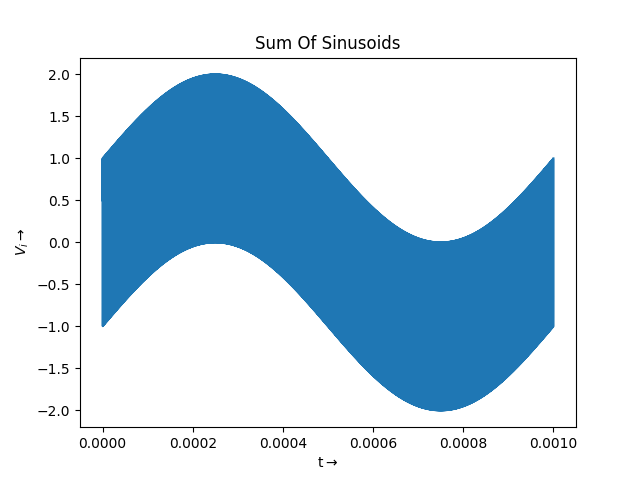
\includegraphics[scale=0.5]{plots/Sum Of Sinusoids.png}   
    \caption{Sum of Sinusoids}
\end{figure}

We first plot the response of the low pass filter in a very short time range and the high pass filter in a very large time range.


\begin{figure}%
    \centering
    \subfloat[\centering Low Pass Filter Circuit]{{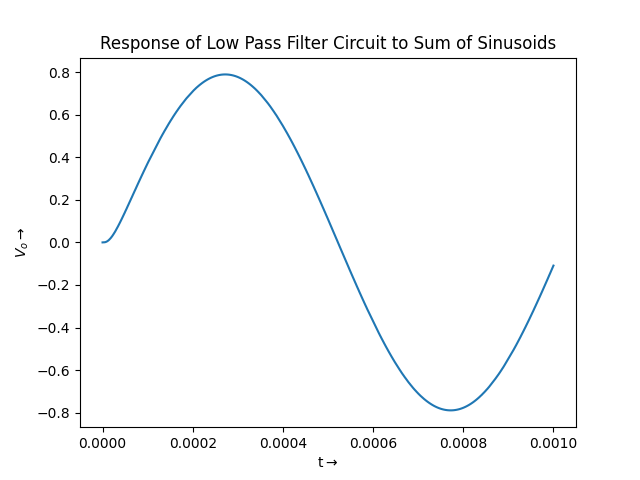
\includegraphics[width=6cm]{plots/Response of Low Pass Filter Circuit to Sum of Sinusoids.png} }}%
    \qquad
    \subfloat[\centering High Pass Filter Circuit]{{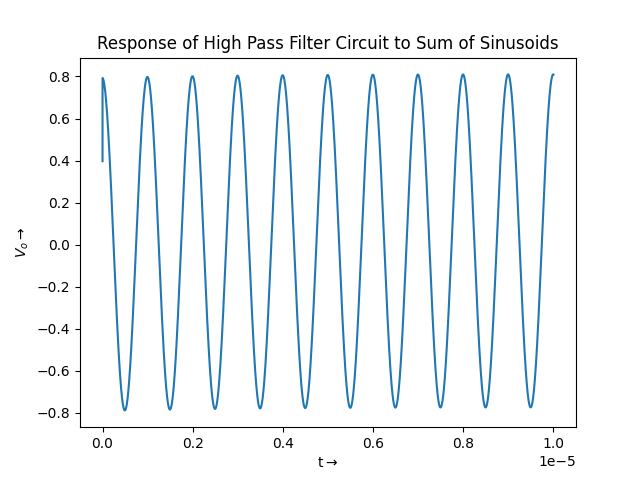
\includegraphics[width=6cm]{plots/Response of High Pass Filter Circuit to Sum of Sinusoids.png} }}%
    \caption{System Response to Sum of Sinusoids}%
    \label{Figure 5}
\end{figure}


\begin{itemize}

    \item
      These time ranges allow us to notice the heavily attenuated part of
      the input better. We can see that an extremely low amplitude high
      frequency sinusoid rides on top of a slow response in the output of
      the low pass filter. This is because the low pass filter has heavily
      attentuated the high frequency component.
    \item
      Similaraly, in the high pass filter, a heavily attenuated low
      frequency sinusoid modulates a high frequency sinusoid. This is
      because the high pass filter highly attenuated the low frequency
      component.

\end{itemize}

\section*{System Response to Damped Sinusoid}

We analyse the Low Pass and High Pass filter using a damped
sinusoid of low frequency and high frequency.

\begin{lstlisting}
def damped_sinusoid(t,decay,freq):
''' Function that gives  a damped sinusoid '''

    return np.cos(freq*t)*np.exp(-decay*t) * (t>0)

\end{lstlisting}

\subsection*{High Frequency Damped Sinusoid}
We analyse the outputs to a high frequency damped sinusoid given as:

\[v_i(t) = \cos(10^7 t) e^{-3000t} u(t)\]

\begin{figure}[!tbh]
    \centering
    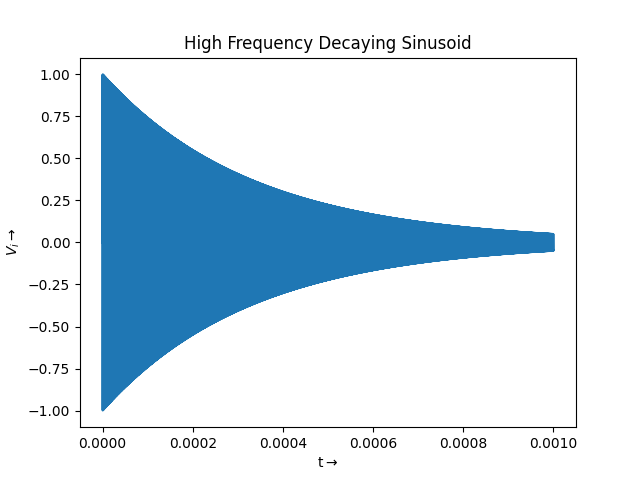
\includegraphics[scale=0.5]{plots/High Frequency Decaying Sinusoid.png}   
    \caption{High Frequency Damped Circuit}
\end{figure}


\begin{lstlisting}

Vi_h = damped_sinusoid(t_h,decay=3e3,freq=1e7)

p=General_Plotter(r't$\rightarrow$',r'$V_{i}\rightarrow$',"High Frequency Decaying Sinusoid")
p.general_plot(t_h,Vi_h)

t,Vo,_ = sp.lsim(H1,Vi_h,t_h)
p=General_Plotter(r't$\rightarrow$',r'$V_{o}\rightarrow$',"Response of Low Pass Filter Circuit to High Frequency Damped")
p.general_plot(t,Vo)

t,Vo,_ = sp.lsim(H2,Vi_h,t_h)
p=General_Plotter(r't$\rightarrow$',r'$V_{o}\rightarrow$',"Response of High Pass Filter Circuit to High Frequency Damped")
p.general_plot(t,Vo)

\end{lstlisting}

\begin{figure}%
    \centering
    \subfloat[\centering Low Pass Filter Circuit]{{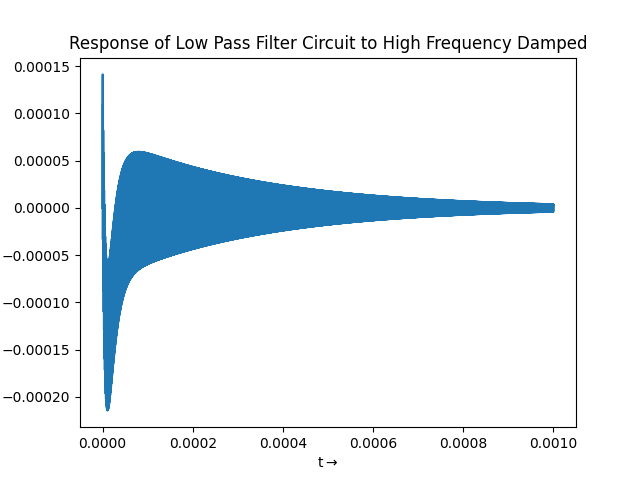
\includegraphics[width=6cm]{plots/Response of Low Pass Filter Circuit to High Frequency Damped.png} }}%
    \qquad
    \subfloat[\centering High Pass Filter Circuit]{{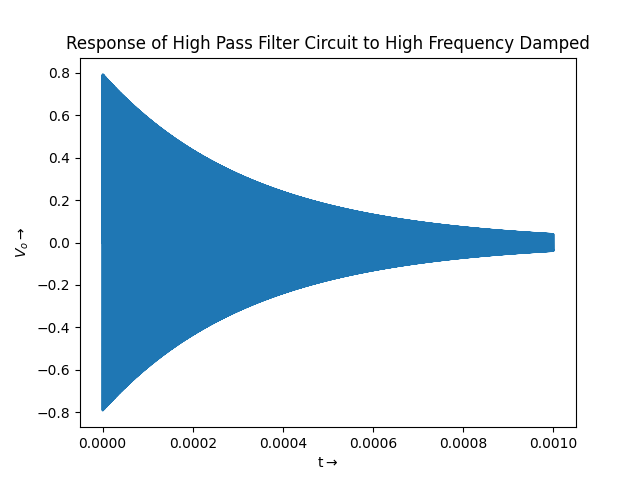
\includegraphics[width=6cm]{plots/Response of High Pass Filter Circuit to High Frequency Damped.png} }}%
    \caption{System Response to High Frequency Damped Sinusoid}%
    \label{Figure 6}
\end{figure}

\begin{itemize}
    \item
      The low pass filter responds fast and heavily attenuates the high
      frequency sinusoid. The output decays as the input also decays.
    \item
      The high pass filter responds by more or less letting the input pass
      through as is, with only a slight attenuation. So the output decays as
      the input does.
\end{itemize}
    

\subsection*{Low Frequency Damped Sinusoid}
We analyse the outputs to a low frequency damped sinusoid given as:

\[v_i(t) = \cos(10^3 t) e^{-10t} u(t)\]

The input waveform is plotted below:

\begin{figure}[!tbh]
    \centering
    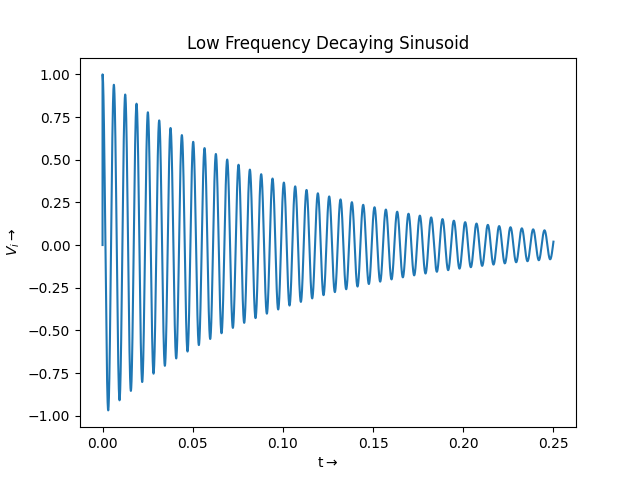
\includegraphics[scale=0.5]{plots/Low Frequency Decaying Sinusoid.png}   
    \caption{Low Frequency Damped Sinusoid}
\end{figure}


\begin{lstlisting}
#Plotting the Low Frequency damped Sinusoid and the response of circuits to this
Vi_l = damped_sinusoid(t_l,decay=1e1,freq=1e3)

p=General_Plotter(r't$\rightarrow$',r'$V_{i}\rightarrow$',"Low Frequency Decaying Sinusoid")
p.general_plot(t_l,Vi_l)

t,Vo,_ = sp.lsim(H1,Vi_l,t_l)
p=General_Plotter(r't$\rightarrow$',r'$V_{o}\rightarrow$',"Response of Low Filter Circuit to Low Frequency Damped")
p.general_plot(t,Vo)

t,Vo,_ = sp.lsim(H2,Vi_l,t_l)
p=General_Plotter(r't$\rightarrow$',r'$V_{o}\rightarrow$',"Response of High Filter Circuit to Low Frequency Damped")
p.general_plot(t,Vo)

\end{lstlisting}

\begin{figure}%
    \centering
    \subfloat[\centering Low Pass Filter Circuit]{{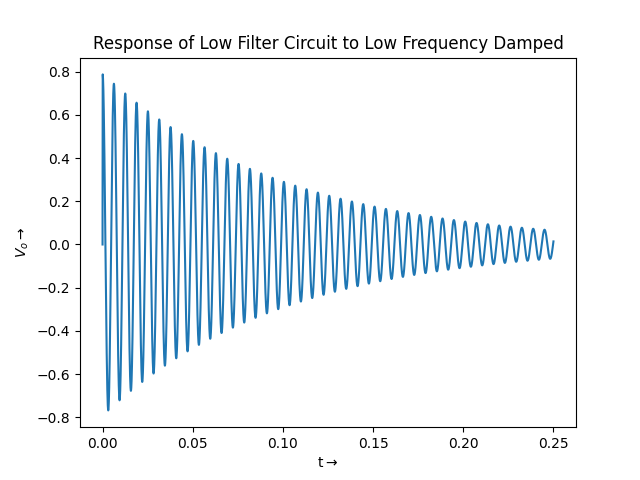
\includegraphics[width=6cm]{plots/Response of Low Filter Circuit to Low Frequency Damped.png} }}%
    \qquad
    \subfloat[\centering High Pass Filter Circuit]{{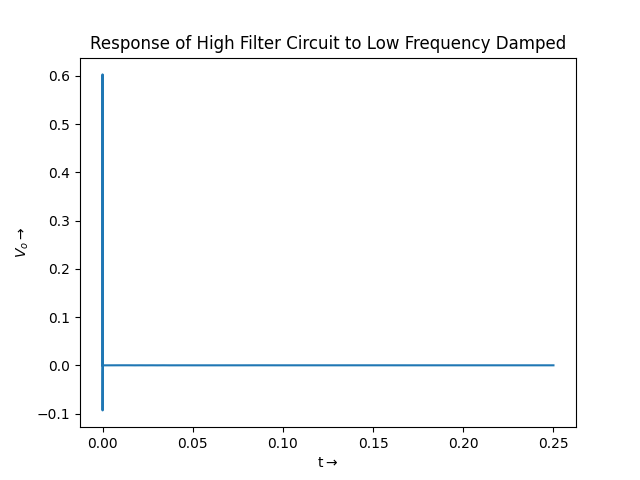
\includegraphics[width=6cm]{plots/Response of High Filter Circuit to Low Frequency Damped.png} }}%
    \caption{System Response to Low Frequency Damped Sinusoid}%
    \label{Figure 7}
\end{figure}




\newpage

\section*{Conclusions}\label{conclusions}

\begin{itemize}
\item
  The low pass filter responds by letting the low frequency sinusoid
  pass through without much additional attenuation. The output decays as
  the input also decays.
\item
  The high pass filter responds by quickly attenuating the input. Notice
  that the time scales show that the high pass filter response is orders
  of magnitudes faster than the low pass response. This is because the
  input frequency is below the cutoff frequency, so the output goes to
  \(0\) very fast.
\item
  In conclusion, the sympy module has allowed us to analyse quite
  complicated circuits by analytically solving their node equations. We
  then interpreted the solutions by plotting time domain responses using
  the signals toolbox. Thus, sympy combined with the scipy.signal module
  is a very useful toolbox for analyzing complicated systems like the
  active filters in this assignment.
\end{itemize}

\end{document}